% Chapter 3

\chapter{State of the Art} % Main chapter title
\label{chap:Chapter3} 

%----------------------------------------------------------------------------------------
\section{Methodology}

\subsection{Research Questions}

RQ1 - Como as frameworks ou bibliotecas disponíveis para desenvolvimento RAG se comparam em termos de arquitetura, flexibilidade e facilidade de utilização?

RQ2 - Quais são os desafios técnicos na implementação de uma solução baseada em RAG para suporte técnico?



RQ3 - Quais as melhores práticas para a indexação e recuperação de dados? 


RQ4 - Qual a LLM mais adequada para uso de RAG para suporte técnico? 




\subsection{Research Scope}

\subsection{Eligibility Criteria}


\subsection{Selection Process}

\subsection{Data Collection}

\section{Results and Analysis}



\subsection{RQ1 - Como as frameworks ou bibliotecas disponíveis para desenvolvimento RAG se comparam em termos de arquitetura, flexibilidade e facilidade de utilização?}

Antes de apresentar cada tecnologia, importa referir que as informações aqui descritas foram obtidas com base na respetiva documentação oficial disponível nos websites de cada projeto. Nesta análise, cada framework será avaliada segundo três critérios: (i) arquitetura, (ii) flexibilidade e (iii) facilidade de utilização. Adicionalmente, serão também consideradas as formas de integração com bases de dados externas (vector stores ou document stores), bem como o suporte e comunidade em torno de cada projeto.


\subsubsection{LangChain}


Fundada por Harrison Chase em 2022, LangChain é uma framework open-source para o desenvolvimento de aplicações que integram LLMs com fontes externas de dados e ferramentas de software. Está disponível em Python e JavaScript, oferecendo um ambiente centralizado e altamente extensível para construir soluções com LLMs de forma modular e reutilizável.

\paragraph{Arquitetura}

A arquitetura do LangChain é baseada no conceito de \textit{Chains}, que representam sequências de chamadas a LLMs e a outras ferramentas auxiliares. Estas \textit{Chains} podem ser compostas de forma modular, permitindo construir fluxos de execução complexos com facilidade.

Com a introdução do LangChain Expression Language (LCEL), passou a ser possível definir estas sequências de forma declarativa. O LCEL oferece diversos construtores prontos para uso, como:

\begin{itemize}
	\item \textit{create\_stuff\_documents\_chain}: Formata uma lista de documentos em um prompt para o LLM.
	\item \textit{create\_sql\_query\_chain}: Gera consultas SQL a partir linguagem natural.
	\item \textit{create\_history\_aware\_retrieve}: Utiliza o histórico de conversas para gerar consultas de busca mais precisas.
	\item \textit{create\_retrieval\_chain}: Integra recuperação de documentos relevantes com geração de respostas por LLM.
\end{itemize}

\subsection{Prompt Templates} TODO retificar esta subsection

São usados para guiar as repostas do modelo reproduzindo um PromptValue. Este é o resultado final da intrução a ser transmitida ao LLM assim que o input do utilizador for executado em cima do template. São importantes pois direcionam a instrução para a obtenção de respostas que vão de em contra ao objetivo da aplicação. 


\begin{lstlisting}[language=Python, caption={Using LangChain to create a prompt template}, label={lst:joke-prompt}]
from langchain_core.prompts import PromptTemplate

prompt_template = PromptTemplate.from_template("Tell me a joke about {topic}")

prompt_template.invoke({"topic": "cats"})
\end{lstlisting}

No contexto de uma aplicação para contar anedotas (\ref{lst:joke-prompt}), apenas com a especificação do tema da anedota, neste caso gatos, o template cria o PromptValue "Tell me a joke about cats"  a ser executado pelo LLM.


https://python.langchain.com/docs/concepts/prompt\_templates/


\paragraph{Flexibilidade}

LangChain é uma das frameworks mais flexíveis atualmente disponíveis. A sua estrutura modular permite criar soluções para diversos domínios — desde sistemas de chat com memória contextual até agentes com raciocínio multi-etapas e integração com APIs externas. Suporta LLMs de múltiplos fornecedores, incluindo:

\begin{itemize} \item OpenAI (via API Key) \item Cohere \item Anthropic (Claude) \item Modelos open-source (como LLaMA, Flan-T5, Mistral, etc.) via Hugging Face \end{itemize}

Os componentes podem ser combinados e substituídos livremente, o que torna o LangChain altamente adaptável a diferentes arquiteturas e necessidades de negócio.

\paragraph{Facilidade de utilização}

A curva de aprendizagem do LangChain pode ser ligeiramente acentuada devido à grande variedade de conceitos e componentes disponíveis. No entanto, a documentação é abrangente e inclui exemplos práticos, tutoriais e guias para casos de uso comuns.

O LCEL veio simplificar bastante o processo de criação de pipelines, ao permitir a definição declarativa de fluxos sem necessidade de escrita de código imperativo detalhado. Ainda assim, o domínio completo da framework pode exigir tempo, especialmente na fase de composição de agentes ou integração de ferramentas externas.

\paragraph{Integração com bases de dados vetoriais e document stores}

LangChain disponibiliza integração nativa com diversos sistemas de armazenamento de documentos, tanto tradicionais como vetoriais, tais como Elasticsearch e Weaviate, duas tecnologias open-source que permitem pesquisa vetorial, armazenamento de embeddings e indexação de documentos.

Estes sistemas são acedidos através de abstrações como \texttt{VectorStoreRetriever} e \texttt{DocumentLoaders}, que permitem a configuração e adaptação do processo de indexação e recuperação de informação de acordo com os requisitos específicos da aplicação.

\paragraph{Suporte e comunidade}

LangChain possui uma comunidade ativa e em crescimento, com elevado dinamismo no repositório GitHub, contanto com mais de cem mil estrelas. A empresa responsável pelo projeto, tem promovido o desenvolvimento contínuo da framework, bem como o lançamento de ferramentas complementares como o LangSmith, destinado à monitorização e depuração de aplicações baseadas em LLMs. Esta vitalidade comunitária traduz-se em documentação continuamente atualizada, partilha regular de boas práticas e integração frequente de contributos externos.


======================================================

https://www.ibm.com/think/topics/langchain
https://python.langchain.com/v0.1/docs/modules/chains/


======================================================



\subsubsection{Haystack}


Haystack é uma framework open-source desenvolvida pela empresa alemã Deepset, com o objetivo de facilitar a construção de pipelines baseadas em LLMs, especialmente para casos de uso como RAG, question answering, classificação, extração de informação e pesquisa semântica em documentos. A linguagem principal utilizada é Python. A primeira versão surgiu em 2020, tendo recentemente evoluído para a versão 2.0, com uma reformulação completa da sua arquitetura.

\paragraph{Arquitetura}

A principal inovação do Haystack 2.0 é a sua arquitetura orientada a componentes. Cada componente representa uma unidade funcional independente, com responsabilidade bem definida dentro de uma pipeline. Estes componentes são combinados de forma declarativa para formar pipelines personalizadas, robustas e escaláveis. Entre os tipos de componentes disponíveis encontram-se:

\begin{itemize} \item \textbf{Document Stores}: responsáveis por armazenar documentos e suportar tanto índices tradicionais quanto vetoriais. \item \textbf{Retrievers}: mecanismos de recuperação de informação, com suporte a métodos tradicionais como BM25 e a recuperação semântica com embeddings. \item \textbf{Rankers}: permitem reordenar os documentos recuperados com base em critérios de relevância mais refinados. \item \textbf{Generators}: utilizam LLMs para gerar respostas com base na informação recolhida. \item \textbf{Prompt Nodes}: enviam prompts configuráveis para modelos locais ou remotos. \item \textbf{Routers}: introduzem lógica condicional nas pipelines, facilitando a criação de fluxos adaptativos. \end{itemize}

As pipelines podem ser definidas em ficheiros YAML ou diretamente em Python, promovendo flexibilidade tanto para utilizadores técnicos como não técnicos.

\paragraph{Flexibilidade}

Haystack destaca-se pela sua grande flexibilidade. A arquitetura baseada em componentes independentes permite a substituição e reconfiguração de cada etapa do fluxo de processamento, facilitando a adaptação a diferentes domínios, fontes de dados e estratégias de interação com LLMs. Os desenvolvedores podem ainda combinar múltiplos retrievers, utilizar lógica condicional com routers e integrar diversos serviços externos com relativa facilidade.

\paragraph{Facilidade de utilização}

A curva de aprendizagem do Haystack pode ser moderada, especialmente para utilizadores que não estejam familiarizados com conceitos como pipelines declarativas ou integração com serviços externos. No entanto, a documentação oficial é bastante completa e a existência de pipelines pré-configuradas — como a \texttt{PredefinedPipeline.INDEXING} e a \texttt{PredefinedPipeline.RAG} — facilita bastante o início do desenvolvimento. Estas permitem, respetivamente, indexar documentos e realizar tarefas de RAG com configuração mínima.

\paragraph{Integração com bases de dados vetoriais/document stores}

Haystack oferece suporte nativo a várias tecnologias de armazenamento de documentos, como Elasticsearch e Weaviate, referidos anteriormente. Em ambiente de desenvolvimento, o Haystack oferece o InMemoryDocumentStore, uma opção lightweight que armazena os documentos diretamente em memória, sendo ideal para testes.

\paragraph{Suporte e comunidade}

Haystack possui uma comunidade ativa. O repositório oficial no GitHub conta com mais de vinte mil estrelas (TODO referencia github), issues frequentemente respondidas, e releases regulares. A documentação é extensa, com guias, tutoriais e exemplos práticos.


======================================================

https://medium.com/aimonks/haystack-an-alternative-to-langchain-carrying-llms-bf7c515c9a7e
https://haystack.deepset.ai/overview/intro
https://docs.haystack.deepset.ai/docs/pipeline-templates



\subsubsection{LlamaIndex}

TODO



\subsubsection{Spring AI}


Spring AI é uma framework recente, disponibilizada publicamente no início de 2024, com o objetivo de simplificar o desenvolvimento de aplicações baseadas em inteligência artificial, especialmente no ecossistema Java. Inspirado por projetos como LangChain e LlamaIndex, o Spring AI surge como uma extensão natural do ecossistema Spring, promovendo a integração de LLMs em aplicações corporativas de forma modular, acessível e escalável.

\paragraph{Arquitetura}

A arquitetura do Spring AI é orientada a componentes e organizada em torno do conceito de \emph{Advisors}, responsáveis por encapsular diferentes estratégias de interação com LLMs e bases de dados vetoriais. A framework disponibiliza dois tipos principais de \textit{advisors} para fluxos RAG:

\begin{itemize} 
        \item \textbf{QuestionAnswerAdvisor}: foca-se na recuperação exata de informação a partir de dados externos, construindo respostas exclusivamente com base nos documentos recuperados da base vetorial. 
        \item \textbf{RetrievalAugmentationAdvisor}: combina a informação externa com o conhecimento prévio embutido no modelo base, permitindo uma resposta enriquecida e mais flexível. 
\end{itemize}

A comunicação com estes componentes é configurada programaticamente através da API do Spring AI, possibilitando a definição de parâmetros como o limiar de similaridade na pesquisa.

Adicionalmente, a framework estrutura os fluxos de processamento em módulos reutilizáveis, entre os quais se destacam: 
\begin{itemize} 
        \item \emph{Document Reader Modules} - para leitura e preparação de documentos; 
        \item \emph{Embedding Modules} - para geração de vetores a partir de texto; \item \emph{Retriever Modules} - para pesquisa em bases vetoriais; 
        \item \emph{LLM Modules} - para interação com o modelo de linguagem. 
\end{itemize}

Esta abordagem modular facilita a composição e manutenção de pipelines RAG personalizadas.

\paragraph{Flexibilidade}

Apesar de ser uma framework emergente, o Spring AI apresenta uma estrutura suficientemente flexível para acomodar diversos casos de uso. A separação clara entre módulos permite que cada fase do pipeline seja configurada ou substituída conforme os requisitos específicos da aplicação.

A framework suporta múltiplos provedores de LLMs, incluindo OpenAI, Hugging Face, Mistral e Cohere, entre outros, com mecanismos de autenticação e configuração standard através do ecossistema Spring.

Por estar profundamente integrado com o ecossistema Spring, a framework beneficia de recursos como injeção de dependências, configuração centralizada, gestão de contexto e integração com outras soluções do universo Spring Boot, o que a torna especialmente atrativa para ambientes corporativos baseados em Java.

\paragraph{Facilidade de utilização}

Um dos principais objetivos do Spring AI é tornar a utilização de LLMs mais acessível a programadores do ecossistema Java. A framework herda a familiaridade e consistência do paradigma Spring, oferecendo uma experiência previsível e bem documentada.

Os \textit{advisors} e módulos podem ser facilmente instanciados e configurados, sendo suportados por exemplos concisos e tutoriais disponíveis na documentação oficial. A integração com ferramentas padrão do Spring (como o Spring Boot Actuator ou o Spring Configuration) facilita a observabilidade e a gestão de parâmetros em ambientes de produção.

Contudo, como se trata de uma framework ainda em evolução, podem existir limitações ao nível de abstrações mais avançadas quando comparada com alternativas mais consolidadas no ecossistema Python.

\paragraph{Integração com bases de dados vetoriais e document stores}

O Spring AI oferece integração nativa com várias bases de dados vetoriais, através da abstração \texttt{VectorStore}. Atualmente, estão disponíveis conectores para:

\begin{itemize} \item \textbf{FAISS} \item \textbf{Qdrant} \item \textbf{Pinecone} \item \textbf{Weaviate} \end{itemize}

Estes armazenamentos vetoriais podem ser utilizados diretamente nos módulos de recuperação, com suporte para parâmetros como o número de documentos a recuperar e o grau de similaridade exigido.

A framework prevê ainda a evolução para incluir mecanismos mais elaborados de pré-processamento de documentos, nomeadamente para segmentação, limpeza e enriquecimento semântico dos conteúdos.

\paragraph{Suporte e comunidade}

Dado o seu lançamento recente, a comunidade do Spring AI ainda se encontra em crescimento. No entanto, beneficia do forte ecossistema da Spring Framework e da extensa base de utilizadores da comunidade Java. O projeto é mantido pela equipa oficial da Spring, o que garante qualidade no design, documentação consistente e ciclos de lançamento regulares.

A documentação oficial cobre os principais casos de uso, e já existem exemplos práticos disponíveis em repositórios públicos que demonstram a aplicação da framework em pipelines RAG.


\subsubsection{Comparação resumo entre tecnologias}


Para resumir, na Tabela \ref{tab:tec-comp} estão descritos os principais pontos de comparação entre as diferentes tecnologias analisadas. 

\begin{table}[H]
        \centering
        \caption{Comparação entre tecnologias RAG}
        \label{tab:tec-comp}
        \renewcommand{\arraystretch}{1.2}
        \begin{tabularx}{\textwidth}{|X|X|X|X|X|X|}
        \hline
        \textbf{Ferramenta} & \textbf{Arquitetura} & \textbf{Flexibilidade} & \textbf{Facilidade de utilização} & \textbf{Integração com bases vetoriais / document stores} & \textbf{Suporte, comunidade e documentação} \\
        \hline
        \textbf{LangChain} & Orquestração modular e declarativa & Elevada & Intermédia &  FAISS, Pinecone, Chroma, Redis, Weaviate, Qdrant. & Comunidade / Suporte \textbf{++} ; Documentação extensa \\
        \hline
        \textbf{Haystack} & Arquitetura orientada a componentes & Elevada & Intermédia a alta & Suporte robusto com "Document Stores" como Elasticsearch, Qdrant, Weaviate; suportando indexação vetorial e tradicional. & Comunidade / Suporte \textbf{+++} ; Documentação extensa \\
        \hline
        \textbf{Spring AI} & Arquitetura modular; integração com o ecossistema Spring. & Moderada a elevada & Alta para programadores Java & FAISS, Qdrant, Pinecone, Weaviate; integração através de "VectorStore". & Comunidade / Suporte \textbf{+} ; Documentação em crescimento  \\
        \hline
        \end{tabularx}
    \end{table}

Em termos de arquitetura as tecnologias são semelhantes em alguns principios gerais, mas diferem na forma como organizam os componentes. A LangChain usa o conceito de chains e agents que permite encadear multiplos passos de forma declarativa. Já a Haystack possui um arquitetura orientada a componentes reutilizáveis. Na Spring AI a arquitetura é modular e integrada no ecossistema Sprint Boot com foco para desenvolvedores Java, usando abstrações típicas do Spring. 


No que diz respeito à flexibilidade, LangChain e Haystack oferecem maior capacidade de personalização, com suporte a múltiplas configurações e integrações. O Spring AI, apesar de mais recente, apresenta uma modularidade sólida, embora mais orientada a padrões corporativos Java.

Em termos de facilidade de utilização, o Spring AI proporciona uma curva de aprendizagem mais suave para programadores familiarizados com Spring Boot. A Haystack combina flexibilidade com pipelines pré-configuradas, ao passo que a LangChain, apesar de poderosa, exige maior domínio técnico para compor soluções complexas.

Todas as ferramentas analisadas oferecem integração com sistemas de armazenamento vetorial da atualidade, como FAISS, Qdrant e Weaviate. O suporte é robusto e adaptável em todas, com destaque para a abstração VectorStore no Spring AI e a diversidade de conectores nativos no Haystack.

Por fim, no que respeita a suporte e comunidade, LangChain e Haystack apresentam ecossistemas consolidados, com documentação extensa, comunidades ativas e evolução contínua — refletido na Tabela \ref{tab:tec-comp} com os níveis \textbf{++} e \textbf{+++}, respetivamente. O Spring AI, embora ainda em fase de maturação, conta com documentação estruturada e o respaldo da comunidade Spring, o que lhe confere um nível \textbf{+} na escala adotada, indicando um bom ponto de partida com potencial de crescimento acelerado.

        

\subsection{RQ2- Quais são os desafios técnicos na implementação de uma solução baseada em RAG para suporte técnico?}

Existem diversos desafios técnicos na implementação de uma solução RAG para suporte técnico, tais como para a indexação e recuperação de dados, a integração com sistemas existentes no sentido de alimentação do conhecimento e precisão e relevância das respostas. 

\subsubsection{Indexação, recuperação e relevância das respostas}

A eficiência do RAG depende da capacidade de recuperar documentação relevante. No contexto de suporte técnico, a recuperação necessita ser precisa para fornecer soluções corretas o que é desafiador devido à complexidade e especificidade da documentação \parencite{ToroIsaza2024}.


No que toca recuperação por similaridades semanticas, \cite{soman2024observations} refere que o uso de embeddings para chunks de texto grandes (> 200 palavras) resulta em valores de similaridade artificialmente altos. Isso sugere que, mesmo quando as frases não são semanticamente parecidas, o modelo acha que são, apenas por serem longas. Contudo, documentação que usa grande número de abreviações e paragrafos para um tópico tornanam as obeservações mais relevantes. Além disso, concluiu-se palavras-chave mais próximas do começo de de uma frase são recuperadas com maior precisão.

Adicionalmente, estudos recentes revelam que sistemas RAG apresentam dificuldades significativas quando aplicados em ambientes empresariais. \textcite{RAGDoesNotWork2024} demonstram que, mesmo quando a resposta correta está presente no contexto, o sistema frequentemente falha em recuperá-la. Isso ocorre, em parte, devido ao desajuste entre a estrutura dos documentos técnicos (como FAQs, procedimentos, logs, etc.) e as estratégias tradicionais de segmentação em chunks.

Essa falha é confirmada por \textcite{SevenPoints2024}, que identificaram múltiplos pontos críticos no funcionamento de sistemas RAG, incluindo:

\begin{itemize}
    \item Falta de conteúdo: Quando a informação necessária não está no contexto, o sistema pode responder com conteúdos enganosos, sugerindo que sabe a resposta mesmo sem dados de apoio.
    \item Fraca classificação da documentação: Mesmo com a informação presente no contexto, ela pode não ser corretamente classificada e consequentemente não recuperada. 
 \item Informação não extraida: Caso haja informações contraditórias no contexto, o retriever pode apresentar falhas.
  \item Especificidade incorreta: O sistema pode gerar respostas muito vagas ou excessivamente específicas sem compreender especificamente o que foi solicitado.
\end{itemize}

Diversas técnicas de Finetunning podem ser utilizadas para contornar estas situações.

TODO melhorar daqui para baixo
Contextos maiores geram respostas mais precisas. A inclusão de metadados, como o nome do ficheiro e número do chunk, melhora a interpretação da informação recuperada. Modelos de embeddings open source também se mostram eficazes, especialmente em textos curtos. Para garantir resultados robustos, é essencial calibrar cuidadosamente o pipeline RAG — incluindo chunking, embeddings, recuperação e consolidação — além de manter uma monitorização contínua, dado que o sistema lida com entradas desconhecidas em tempo real.



\subsubsection{Integração com Sistemas Existentes}




https://arxiv.org/pdf/2409.13707

https://arxiv.org/pdf/2404.00657


\section{Trabalhos Relacionados}

TODO incluir isto?: Embora o foco desta dissertação seja a aplicação de RAG em contextos de suporte técnico, são também analisados trabalhos em domínios adjacentes quando estes oferecem contributos relevantes em termos de arquitetura, avaliação ou boas práticas.

\subsection{Análise Individual}

\subsubsection{RAG Chatbot para a OptiMicro Technologies}

A OptiMicro, empresa de software Canadiana, decidiu apostar no desenvolvimento de um chatbot utilizando RAG para melhorar o seu serviço de apoio técnico da empresa, mais especificamente no seu serviço DentalWare.

O software foi desenvolvido através de uma plataforma lowcode denominada Flowise AI e a sua arquitetura consistiu em três fases principais: indexação, recuperação e geração. Na fase de indexação, foram utilizados registos de suporte técnico e manuais do software DentalWare, segmentados em chunks de texto. Os dados foram convertidos em vetores através do modelo all-MiniLM-L6-v2, acedido via API da HuggingFace, e armazenados numa base de dados vetorial Pinecone, escolhida pela sua elevada performance. Na etapa de recuperação, a query do utilizador é embedded com o mesmo modelo e comparada com os vetores indexados, sendo selecionados os segmentos mais relevantes. Por fim, a resposta é gerada com o modelo LLaMA 2 (7B), executado localmente via Ollama. 

Esta arquitetura encontra-se descrita no diagrama da Figura \ref{fig:opti-micro-arch}, onde é possível verificar de que forma os componentes se relacionam. É de notar que foram utilizados dois documentos como fonte de informação externa definidos de forma estática, tornando o software um pouco restrito.

\begin{figure}[H]
        \centering
        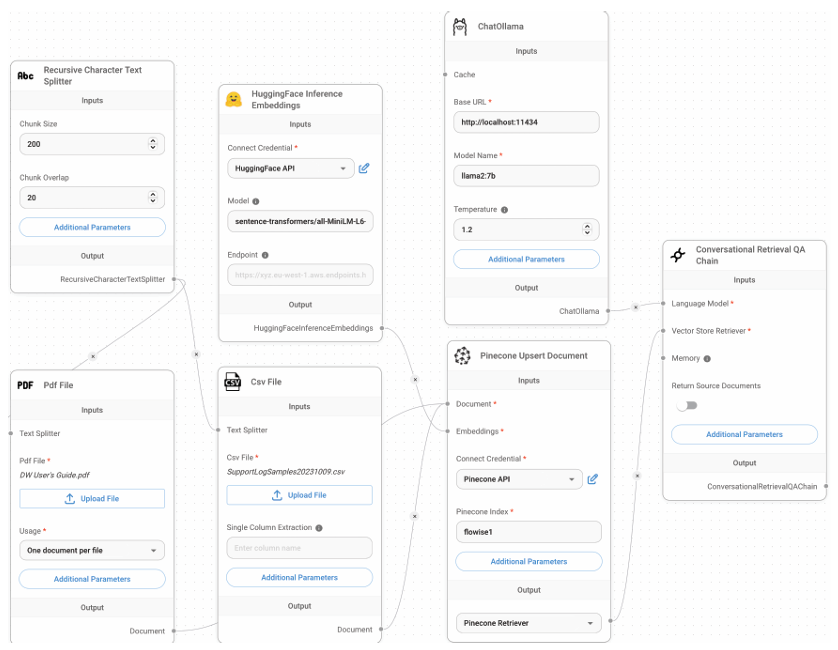
\includegraphics[width=1\linewidth]{ch3/assets/optimicro-arch.png}
        \caption{Arquitetura do chatbot RAG da OptiMicro \parencite{lee2024development}}
        \label{fig:opti-micro-arch}
\end{figure}


Para avaliar o desempenho do chatbot, foram utilizadas 75 questões reais relacionadas com suporte técnico ao software DentalWare. As respostas geradas por este chatbot foram comparadas com as de um chatbot LLM genérico, tendo ambas sido avaliadas com base nos critérios de ROUGE (ROUGE-1, ROUGE-2 e ROUGE-L) e por humanos da OptiMicro. Os resultados demonstraram que o chatbot RAG obteve melhores pontuações em todas as métricas ROUGE, destacando-se com aumentos de 38\%, 18\% e 40\%, respetivamente, face ao modelo genérico, o que evidencia uma maior fidelidade aos conteúdos técnicos. Na avaliação humana, o chatbot RAG obteve 20 respostas classificadas como boas, 18 como razoáveis e apenas 2 como fracas, enquanto o LLM genérico apresentou apenas 3 boas respostas e 2 razoáveis, totalizando 70 respostas consideradas fracas. Estes resultados confirmam a superioridade do modelo RAG no contexto de apoio técnico, pela sua capacidade de gerar respostas mais relevantes e alinhadas com os dados específicos da empresa.



TODO ponto negativa deste software: não foi implementado mecanismo para atualizar automaticamente a base de dados vetorial consoante updates na documentação


\subsubsection{Sistema RAG de Recomendação para Suporte Técnico} 

\cite{isaza2024retrieval} propuseram um sistema de recomendação para resolução de incidentes em suporte técnico baseado em RAG, com o objetivo de sugerir soluções fundamentadas em documentação.


A arquitetura do sistema encontra-se representada na Figura \ref{fig:ticket-recomendation-rag}, sendo composta por cinco etapas principais. A primeira é o pré-processamento, onde certas características do incidente são normalizadas e comparadas com siglas ou nomes alternativos, de forma a melhorar a query de recuperação. Segue-se a classificação de tickets, através do classificador transformer IBM Slate 125m, onde o assunto e a descrição do incidente são analisados para determinar se a sua resolução é viável apenas com a informação fornecida — casos denominados single-turn. Caso o ticket não seja classificado como single-turn, a pipeline termina imediatamente.
As etapas seguintes consistem na geração de uma query concisa a partir do conteúdo do ticket, seguida da recuperação com reranking, onde são selecionados os três documentos mais relevantes a partir de uma base de dados vetorial Milvus. A resposta final é gerada com base nesses documentos e é acompanhada de links para as fontes consultadas.

\begin{figure}[H]
        \centering
        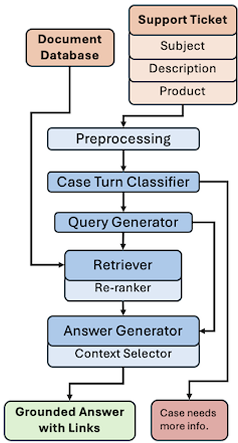
\includegraphics[width=0.3\linewidth]{ch3/assets/ticket-recomendation-rag.png
        }
        \caption{Arquitetura do sistema de recomendação de resolução de incidentes proposto por  \cite{isaza2024retrieval}}
        \label{fig:ticket-recomendation-rag}
\end{figure}


O sistema foi testado em diversos aspetos, quer na geração de queries ou quer na geração da respostas, tendo sido utlizados diferentes LLMs para cada vertente. O modelo Mixtral 8x7B Instruct, que é um LLM fine-tuned para interações dialogadas como chatbots, obteve um BertScore F1 de 0,91 na tarefa de normalizar incidentes em queries concisas, semelhante a LLMs maiores como Falcon-40B, porém com menor custo computacional. Na geração de respostas, este mesmo modelo, combinado com RAG, superou o GPT-4 em métricas como ROUGE-L F1 (0,41 vs. 0,34) e BertScore (0,87 vs. 0,86), destacando a eficienciencia de modelos menores com contexto recuperado. Os autores destacaram também que modelos fine-tuned com infusão de conhecimento técnico, como o modelo InstructLab-IT (7 mil milhões parâmetros), podem superar modelos de grande porte para casos gerais. 



\subsubsection{Fabula}

ficheiro fabula.pdf nas transferencias
não é relacionado com IT support mas se calhar é interessante incluir para demonstrar outro caso de uso do RAG e pode dar algum insight util

\subsection{Conclusões}





